% Latex document @author Clemens Näther, Jakub Kliemann, s85426, s85515
%--------------------------------------------------------------------
\documentclass[a4paper,12pt]{article}
\usepackage[utf8]{inputenc}
\usepackage{graphicx}
\usepackage[hidelinks]{hyperref}
\usepackage{float}
\usepackage{listings}
\usepackage{color}
\usepackage{amsmath}
\usepackage{pdfpages}
\usepackage{fancyhdr}
\usepackage{lastpage}
\usepackage{geometry}
\usepackage{listings}
\usepackage{xcolor}
\usepackage{mhchem}
\usepackage{comment}

\usepackage{biblatex} % Verwende BibLaTeX
\addbibresource{bibliography.bib} % Deine .bib-Datei

\lstset{ %
  language=,
  basicstyle=\ttfamily\small,
  backgroundcolor=\color{lightgray!20},
  frame=single,
  columns=fullflexible,
  breaklines=true,
  captionpos=b
}

\geometry{a4paper, top=25mm, left=30mm, right=25mm, bottom=30mm,
headsep=10mm, footskip=12mm}

\pagestyle{fancy}

\lhead{Dokumentation}

\rhead{Seite \thepage\ von \pageref{LastPage}}

\cfoot{}

\renewcommand{\headrulewidth}{0.4pt}

\renewcommand{\footrulewidth}{0.4pt}

\begin{document}

\begin{titlepage}

\begin{center}


\includegraphics[height=4cm]{../images/htwd-logo.jpg}\\[1cm]

\textsc{\LARGE Hochschule für Technik und Wirtschaft}\\[1.5cm]

\textsc{\Large Dokumentation}\\[0.5cm]

% Title
\newcommand{\HRule}{\rule{\linewidth}{0.5mm}}
\HRule \\[0.4cm]
{ \huge \bfseries \textsc{Projektseminar}}\\[0.4cm]
{ \huge \bfseries \textsc{Optimierung und Unsicherheitsquantifizierung mit Bayesianischer Statistik und MCMC-Methoden}}\\[0.4cm]
{ \huge \bfseries \textsc{(Prof. Schwarzenberger)}}\\[0.4cm]
\HRule \\[1.5cm]

% Author and supervisor
\begin{minipage}{0.4\textwidth}
\begin{flushleft} \large

\emph{Clemens Näther, s85426}\\
\emph{Jakub Kliemann, s85515}\\

\end{flushleft}
\end{minipage}
\end{center}
\end{titlepage}

\tableofcontents
\newpage

\section{Einleitung}
Die Statistik ist ein wesentlicher Bestandteil der Wissenschaft. Sie ermöglicht es, aus Daten Informationen zu gewinnen und aus diesen Schlussfolgerungen zu ziehen. Es exsistieren dabei aber zwei verschiedene Ansätze, die klassische und die bayesianische Statistik. Beide bieten unterschiedliche Perspektiven und Werkzeuge zur Analyse und Interpretation von Unsicherheiten, und die Entscheidung für eine Methode kann erhebliche Auswirkungen auf die Schlussfolgerungen einer Studie haben.\\\\
In dieser Arbeit liegt der Fokus auf der bayesianischen Statistik, einem Ansatz, der die Wahrscheinlichkeit als subjektives Maß für die Unsicherheit interpretiert und es ermöglicht, Vorwissen systematisch in den Analyseprozess einzubringen. Der Vergleich mit der klassischen Statistik, die auf der relativen Häufigkeit basiert, zeigt, wie unterschiedlich die Ansätze sowohl in der Theorie als auch in der Praxis sind.\\\\
Ein zentraler Schwerpunkt der Arbeit liegt darin die theoretischen Grundlagen der bayesianischen Statistik zu erläutern und den Prinzipien der klassischen Statistik gegen-überzustellen. Dabei soll insbesondere auf die Markov Chain Monte Carlo (MCMC) Methoden eingegangen werden, die es ermöglichen, komplexe Modelle zu schätzen und zu simulieren. Inbesondere wird der Metropolis-Hastings-Algorithmus, einer der bekanntesten Algorithmen zur Erstellung von Markovketten vorgestellt.\\\\
Anschließend wird im zweiten Teil der Arbeit die praktische Anwendung der bayesianischen Statistik und der MCMC-Methoden anhand von Beispielen und Datensätzen in Python demonstriert. Dabei wird gezeigt, wie bayesianische Modelle implementiert und auf verschiedene Datensätze angewendet werden können. Die Ergebnisse werden interpretiert und mit klassischen Methoden verglichen.\\\\
\newpage

\section{Theoretischer Teil}

\subsection{Grundlagen der bayesianischen Statistik und das Bayes'sche Theorem}
\subsubsection{Einführung in die bayesianische Statistik}

Die bayesianische Statistik ist ein Zweig der Statistik. Sie unterscheidet sich im wesentlichen in der Interpretation der Wahrscheinlichkeit von der klassischen Statistik. Die klassische Statistik definiert die Wahrscheinlichkeit als die \textbf{relative Häufigkeit} in einem Zufallsexperiment \parencite[2]{StatistikKlassischOderBayes}. In der bayesianischen Statistik hingegen wird die Wahrscheinlichkeit als Grad des Glaubens respektiv als \textbf{Plausibilität} eines Ereignisses oder einer Aussage interpretiert \parencite[1]{EinfBayesStatistik}. \\\\
Kern der bayesianischen Statistik ist es Wissen über ein Ereignis zu verfeinern, sobald neue Informationen vorliegen. Dazu nutzt man hauptsächlich das \textbf{Bayes'sche Theorem}, welches erlaubt das Vorwissen (Prior) mit neuen Daten (Likelihood) zu kombinieren und daraus eine aktualisierte Wahrscheinlichkeit (Posterior) zu berechnen. \\\\
Mit Hilfe des Bayes'schen Theorems kann man unbekannte Parameter schätzen, ein Konfidenzintervall für diese Parameter angeben und Hypothesen prüfen. Die klassische Statistik benötigt hingegen dafür Testgrößen, weshalb die bayesianische Statistik als flexibler und intuitiver gilt. \parencite[1]{EinfBayesStatistik}. \\\\
Problem der bayesianischen Statistik ist jedoch, dass die Berechnung der Posterioriverteilung analytisch oft nicht möglich ist. Da es nun aber gute numerische Methoden wie die \textbf{Markov Chain Monte Carlo (MCMC)} Methoden gibt, findet die bayesianische Statistik immer mehr Anwendungen. So zum Beispiel in der Medizin oder für künstliche Intelligenzen. \parencite[1]{StatistikKlassischOderBayes}.

\subsubsection{Das Bayes'sche Theorem und seine Bestandteile}

Das Bayes'sche Theorem ist ein fundamentales Konzept der bayesianischen Statistik.Es beschreibt, wie man vorhandenes Vorwissen durch neue Daten aktualisiert. \\\\
Die \textbf{Prioriverteilung} beschreibt die anfänglichen Annahmen oder das Vorwissen über einen 
Parameter oder ein Ereignis, bevor neue Daten berücksichtigt werden.
Dabei ``enthält die Priorverteilung eines Parameters $\theta$, ausgedrückt durch f ($ \theta $), 
was man vor Auswertung der Stichprobe über $\theta$ weiß.'' \parencite[90]{StatistikKlassischOderBayes}. \\
Als Priori-Wahrscheinlichkeit wird somit die Wahrscheinlichkeit $ P(A) $ bezeichnet. \\\\
Die \textbf{Posterioriverteilung} beschreibt das Wissen über einen Parameter oder ein Ereignis, nachdem alle 
vorhandenen Daten berücksichtigt wurden. Durch die neuen Daten, meist einer Stichprobe, wird die 
anfängliche Annahme, die durch die Prioriverteilung ausgedrückt wird, aktualisiert. 
Dies führt zu einer neuen Verteilung die widerspiegelt, wie wahrscheinlich verschiedene Werte 
des Parameters auf Grundlage sowohl des Vorwissens als auch der neuen Informationen sind. \parencite[109]{StatistikKlassischOderBayes}\\
Die Posteriori-Wahrscheinlichkeit wird somit als $ P(A|B) $ bezeichnet. \\\\
Die \textbf{Likelihood-Funktion} enthält die Informationen, die die Daten über den Parameter oder das Ereignis liefern.
Dabei beschreibt die Likelihood die Informationen aus den neuen Daten, die zur Aktualisierung der Prioriverteilung beitragen. \parencite[88]{StatistikKlassischOderBayes}\\
Die Likelihood-Wahrscheinlichkeit wird somit als $ P(B|A) $ bezeichnet. \\\\
Die Wahrscheinlichkeit $ P(B) $ wird als Normierungskonstante bezeichnet. Sie sorgt dafür, 
dass die Posterioriverteilung korrekt normiert ist, das heißt, dass die Summe der 
Wahrscheinlichkeiten aller möglichen Werte des Parameters 1 ergibt. \parencite[109]{StatistikKlassischOderBayes} \\\\
Das Bayes'sche Theorem lässt sich somit wie folgt darstellen:
\begin{equation}
P(A|B) = \frac{P(A) \cdot P(B|A)}{P(B)}
\end{equation}
Das Bayes'sche Theorem lässt sich auch rekursiv anwenden \parencite[17]{EinfBayesStatistik}. \\
Gegeben sei das Ereignis $A$ sowie die Teilergebnisse $B_1, B_2, ..., B_n$. Dann ergibt sich die Wahrscheinlichkeit $P(A|B_1)$ zu:
\begin{equation}
P(A|B_1) = \frac{P(A) \cdot P(B_1|A)}{P(B_1)}
\end{equation}
Nun wird die Information $B_2$ hinzugefügt. Die Wahrscheinlichkeit $P(A|B_1, B_2)$ ergibt sich bei Unabhängigkeit von den Teilereignissen $B_1, B_2, ..., B_n$ zu:
\begin{equation}
P(A|B_1, B_2) = \frac{P(A) \cdot P(B_1|A) \cdot P(B_2|A)}{P(B_1) \cdot P(B_2)}
\end{equation}
Weiterhin lässt sich diese Formel umstellen, wodurch deutlich wird, dass beim Hinzufügen von neuen Informationen die Posterioriverteilung aktualisiert wird:
\begin{equation}
P(A|B_1, B_2) = \frac{P(A) \cdot P(B_1|A) \cdot P(B_2|A)}{P(B_1) \cdot P(B_2)} = P(A|B_1) \cdot \frac{P(B_2|A)}{P(B_2)}
\end{equation}
Dies lässt sich allgemein formulieren für:
\begin{equation}
P(A|B_1, B_2, ..., B_n) = P(A|B_1, B_2, ..., B_{n-1}) \cdot \frac{P(B_n|A)}{P(B_n)}
\end{equation}
Die Wahl der Prioriverteilung ist ein wichtiger Aspekt der bayesianischen Statistik. Sie wird immer so gewählt, dass die Entropie maximal ist. Die Entropie ist ein Maß für die Unsicherheit, was bedeutet, dass nur Informationen enthalten sind, die vor der Beobachtung bekannt sind. \parencite[57]{EinfBayesStatistik}. Unter folgenden Bedingungen ist die Prioriverteilung optimal \parencite[59]{EinfBayesStatistik}:
\begin{itemize}
  \item Zufallsvariablen, die in $[a,b]$ definiert sind, sind \textbf{gleichverteilt}
  \item Zufallsvariablen mit gegebenen Mittelwert und Varianz sind \textbf{normalverteilt}
  \item Zufallsvariablen mit gegebenen Mittelwert sind \textbf{exponentialverteilt}
  \item Zufallsvariablen mit gegebenen Mittelwert und Varianz im Intervall [0,$\infty$] besitzen eine \textbf{abgeschnittene Normalverteilung}
\end{itemize}
Wenn keine Informationen über den Parameter vorliegen, wird eine \textbf{uninformative} Prioriverteilung gewählt. Es handelt sich dabei um eine uneigentliche Verteilung. \parencite[57]{EinfBayesStatistik}.

\subsubsection{Beispiele und praktische Anwendungen}
\textbf{Beispiel 1}: $m$ gleichgeformte Kugeln, unter denen sich $k$ rote Kugeln und $m-k$ schwarze Kugeln befinden. Eine Kugel wird zufällig gezogen. 
Die Wahrscheinlichkeit, dass die gezogene Kugel rot ist, beträgt 
\begin{equation}
P(A) = \frac{k}{m} = p
\end{equation}
Der Versuch wird erweitert, sodass $n$-mal eine Kugel mit Zurücklegen gezogen wird.
Die Wahrscheinlichkeit, dass $x$-mal eine rote Kugel bie $n$-maligem Ziehen gezogen wird,
beträgt
\begin{equation}
P(x|n,p) = \binom{n}{x} \cdot p^x \cdot (1-p)^{n-x}
\end{equation}
Sei nun $p$ unbekannt. Dieses $p$ ist nun zu schätzen.
Die Binomialverteilung wird nun als Likelihood-Funktion verwendet:
\begin{equation}
P(n,x|p) = \binom{n}{x} \cdot p^x \cdot (1-p)^{n-x}
\end{equation}
wobei $0 \leq p \leq 1$.
Als Prioridichte wird die Gleichverteilung verwendet, da es keine Informationen über $p$ gibt.
\begin{equation}
  P(p) =
  \begin{cases}
    1, & \text{für } 0 \leq p \leq 1 \\
    0, & \text{sonst}
  \end{cases}
\end{equation}
Die Posterioridichte ergibt sich somit zu:
\begin{equation}
P(p|n,x) = \frac{\binom{n}{x}  p^x \cdot (1-p)^{n-x}}{P(n,x)}
\label{eq:posterior}
\end{equation}
Vergleicht man dies mit der Dichtefunktion der Beta-Verteilung, so erkennt man dass die Posterioridichte einer Beta-Verteilung entspricht.
\begin{equation}
P(p|n,x) = \frac{(n+1)!}{x!\cdot(n-x)!} \cdot p^x \cdot (1-p)^{n-x}
= \frac{\Gamma(n+1)}{\Gamma(x+1)\cdot\Gamma(n-x+1)} \cdot p^x \cdot (1-p)^{n-x}
\end{equation}
Somit suche nach Maximum der Posterioridichte, um den Schätzer für $p$ zu finden.
\begin{equation}
\frac{d}{dp} P(p|n,x) = xp^{x-1} \cdot (1-p)^{n-x} - (n-x)p^x \cdot (1-p)^{n-x-1} = 0
\end{equation}
\begin{equation}
\Rightarrow xp^{x-1} \cdot (1-p)^{n-x} = (n-x)p^x \cdot (1-p)^{n-x-1}
\end{equation}
Vereinfacht ergibt sich:
\begin{equation}
\Rightarrow x(1-p) = (n-x)p
\end{equation}
\begin{equation}  
\Rightarrow \frac{x}{p} - \frac{n-x}{1-p} = 0
\end{equation}
\begin{equation}
\Rightarrow p = \frac{x}{n}
\end{equation}
Der Schätzer für $p$ ist somit der relative Anteil der roten Kugeln an der Gesamtanzahl der Kugeln. \\\\
\textbf{Beispiel 2}: Beispiel 1 wird erweitert. Es wird nun eine zweite Stichprobe gezogen. 
Stichprobe 1: $n_1 = 10$, $x_1 = 4$, Stichprobe 2: $n_2 = 20$, $x_2 = 6$.
Daten sind unabhängig voneinander. Die Daten (Posterioriverteilung) der 1. Stichprobe dienen nun
als Prioridichte für die 2. Stichprobe. Man erhält somit:
\begin{equation}
P(p|n_1,x_1,n_2,x_2) = \frac{P(p|n_1,x_1) \cdot P(p|n_2,x_2)}{P(n_1,x_1,n_2,x_2)}
\end{equation}
Dabei ist die Prioridichte identisch zur Posterioridichte der 1. Stichprobe, siehe Gleichung \eqref{eq:posterior}.
Die Posterioridichte der 2. Stichprobe ergibt sich somit zu:
\begin{equation}
P(p|n_1,x_1,n_2,x_2) = \frac{\binom{n_1+n_2}{x_1+x_2} \cdot p^{x_1} \cdot (1-p)^{n_1-x_1} \cdot p^{x_2} \cdot (1-p)^{n_2-x_2}}{P(n_1,x_1,n_2,x_2)}
\end{equation}
Oder mithilfe der Beta-Verteilung:
\begin{equation}
  P(p|n_1,x_1,n_2,x_2) = \frac{\Gamma(n_1+n_2+1)}{\Gamma(x_1+x_2+1)\cdot\Gamma(n_1+n_2-x_1-x_2+1)} \cdot p^{x_1+x_2} \cdot (1-p)^{n_1+n_2-x_1-x_2}
\end{equation}
Die Daten der 1. und 2. Stichprobe könnnen somit kombiniert werden.
Für die Daten $n_1 = 10$, $x_1 = 4$, $n_2 = 20$, $x_2 = 6$:
\begin{equation}
P(p|10,4,20,6) = 931 395 465p^{10} \cdot (1-p)^{20}
\end{equation}

\subsubsection{Punktschätzer, Konfidenzintervalle und Hypothesenprüfung in der bayesianischen Statistik}
\subsection*{\underline{Punktschätzer}}
Im folgenden wird die Schätzung eines Parameters mithilfe der Bayes-Strategie erläutert. \\
Die möglichen Schätzwerte der Parameter $x$ werden als $\hat{x}$ bezeichnet. Die wahren Parameter werden als $x$ bezeichnet. \\
Es wird eine Kostenfunktion $L(\hat{x},x)$ definiert, die die Kosten für die Schätzung $\hat{x}$ des wahren Parameters $x$ angibt.
Dies bedeutet, dass die Kostenfunktion die Differenz zwischen dem wahren Parameter $x$ und der Schätzung $\hat{x}$ angibt.
Dabei gibt es verschiedene Kostenfunktionen, die verwendet werden können. \parencite[65]{EinfBayesStatistik} \\\\
Die \textbf{quadratische Kostenfunktion} ist definiert als: $L(x-\hat{x}) = (x-\hat{x})\Sigma^{-1}(x-\hat{x})$. \\
Diese gibt den quadratischen Abstand zwischen dem wahren Parameter $x$ und der Schätzung $\hat{x}$ an.
Die zu erwartenden Kosten werden berechnet mit dem Erwartungswert der Kostenfunktion.
Diese Schätzung führt zu dem Erwartungswert von $x$, das heißt $\hat{x} = E(x)$. \parencite[65-66]{EinfBayesStatistik} \\\\
Die \textbf{Kostenfunktion der absoluten Fehler} ist definiert als: $L(x,\hat{x}) = |x-\hat{x}|$.
Diese gibt den absoluten Abstand zwischen $x$ und $\hat{x}$ an.
Die Schätzung mit dem absoluten Fehler ergibt den Median der Verteilung, das heißt $F(\hat{x}_{med}) = 0.5$ \parencite[67-68]{EinfBayesStatistik} \\\\\\\\
Die \textbf{Null-Eins-Kostenfunktion} bedeutet, dass es entweder Kosten oder keine Kosten gibt.
Diese ist definiert durch: $L(x-\hat{x}) = 
\begin{cases}
  0 & \text{für } |x-\hat{x}| < b \\
  a & \text{für } |x-\hat{x}| \geq b
\end{cases}$,\\
wobei $a$ und $b$ als Konstaten angenommen werden. Wenn der Fall $b \to 0$ betrachtet wird,
ergibt sich als Schätzer das Argument des Maximums der Posterioriverteilung, das heißt $\hat{x}_M = \arg \max \; p(x|y)$. \parencite[68-69]{EinfBayesStatistik}\\\\
Es ist so ersichtlich, dass es verschiedene Punktschätzer in der bayesianischen Statistik gibt:
\begin{itemize}
  \item \textbf{Erwartungswert} $\hat{x} = E(x)$
  \item \textbf{Median} $\hat{x} = x_{0.5}$
  \item \textbf{Maximum der Posterioriverteilung} $\hat{x} = \arg \max \; p(x|y)$
\end{itemize}
Die Wahl zwischen den Schätzern hängt so von der Problemstellung ab.

\subsection*{\underline{Konfidenzintervalle}}
Um Unsicherheiten bei Schätzungen zu quantifizieren werden oftmals \textbf{Konfidenzintervall} verwendet. Konfidenzintervalle geben einen Bereich an, in dem ein unbekannter Parameter mit einer bestimmten Wahrscheinlichkeit liegt. In der Bayes Statistik kann eine Bereichschätzung unmittelbar aus der Posterioriverteilung abgeleitet werden. \parencite[71]{EinfBayesStatistik} \\\\
Wenn P(x$|$y) die Posterioridichte für den Parameter x ist, ist das Konfidenzintervall mit Konfidenzniveau 1-$\alpha$ definiert als:
\begin{equation}
  P(x \in X_u|y) = \int_{X_u} P(x|y) dx = 1-\alpha
\end{equation}
Wobei für alle $x_1 \in X_u, x_2 \not\in X_u$ gilt $P(x_1|y) \geq P(x_2|y)$; Xu ist dabei ein Unterraum auf dem Parameterraum \parencite[71]{EinfBayesStatistik}. Meist wird für $\alpha$ 0.1, 0.05 oder 0.01 gewählt. Höhere Konfidenzniveaus führen zu größeren Intervallen, da mehr Unsicherheit abgedeckt wird, während niedrigere Konfidenzniveaus kleinere Intervalle liefern, die jedoch ein höheres Risiko haben, den wahren Parameter nicht einzuschließen. \\\\
Falls die Posterioriverteilung P(x$|$y) beispielsweise der Normalverteilung N($\mu,\sigma^2$) ent- spricht, ist das Konfidenzintervall symmetrisch um den Mittelwert und die Grenzen lassen sich einfach durch die Quantile der Standardnormalverteilung z über $\mu - z_{1-\alpha/2} * \sigma$ und $\mu + z_{1-\alpha/2} * \sigma$ bestimmen.\\\\
Da die Konfidenzintervalle in der bayesianischen Statistik auf der Posterioriverteilung basieren, unterscheiden sich die Ergebnisse von denen der klassischen Statistik, da diese auf einer anderen Grundlage definiert sind.

\newpage
\subsection*{\underline{Hypothesenprüfung}}
Hypothesenprüfung ist eine Methode, mit der man Annahmen über unbekannte Parameter überprüft. Dabei wird entschieden, ob solche Annahmen akzeptiert oder abgelehnt werden sollen. \parencite[74]{EinfBayesStatistik}. Man unterscheidet zwischen der Nullhypothese $H_0$ und der Alternativhypothese $H_1$. Die Nullhypothese ist die Annahme, die überprüft wird, während die Alternativhypothese die Annahme ist, die akzeptiert wird, wenn die Nullhypothese abgelehnt wird. \\\\
In der bayesianischen Statistik werden Hypothesen durch Unterräume des Parameterraums definiert. Seien $X_1$ und $X_2$ disjunkte Unterräume des Parameterraums, so lauten die Hypothesen $H_0: x \in X_1$ und $H_1: x \in X_2$. Die Wahrscheinlichkeiten für diese Hypothesen ergeben sich direkt aus der Posterior-Dichte. Die Wahrscheinlichkeit, dass die Nullhypothese wahr ist, lautet:
\begin{equation}
  P(H_0|y) = \int_{X_1} P(x|y) dx
\end{equation}
Analog gilt dies für $P(H_1|y)$ \parencite[74]{EinfBayesStatistik}. Ist jetzt $P(H_0|y) > P(H_1|y)$ rsp. $\frac{P(H_0|y)}{P(H_1|y)}>1$, so wird die Nullhypothese akzeptiert, andernfalls die Alternativhypothese. \parencite[77]{EinfBayesStatistik}. \\\\
Bei einer Punkthypothese $H_0: x = x_0$ ergibt sich $P(H_0|y) = 0$, da die Posterior-Dichte kontinuierlich ist und ein einzelner Punkt daher keine Wahrscheinlichkeit besitzt. In solchen Fällen greift man beispielsweise auf Konfidenzintervalle zurück: Liegt der Wert $x_0$ innerhalb des Konfidenzintervalls, wird die Nullhypothese akzeptiert, andernfalls abgelehnt \parencite[84]{EinfBayesStatistik}. \\\\
Ein wesentlicher Unterschied zur klassischen Statistik besteht darin, dass in der traditionellen Hypothesenprüfung die Nullhypothese solange als gültig angesehen wird, bis genügend Beweise dagegen vorliegen (Prinzip des Zweifelns). In der bayesianischen Statistik hingegen werden die Wahrscheinlichkeiten beider Hypothesen direkt geschätzt, wodurch beide Hypothesen von Anfang an gleichberechtigt betrachtet werden. \parencite[83]{EinfBayesStatistik}.


\newpage

\subsection{Markov Chain Monte Carlo (MCMC) Methoden}
\subsubsection{Einführung in MCMC-Methoden}
Bei einer direkten Simulation wird vorrausgesetzt, dass die Verteilung der Zufallsvariablen bekannt ist.
Dies ist jedoch in der Praxis nicht immer gegeben.
Die Berechnung der Posterioriverteilung ist analytisch oft nicht möglich, vor allem bei komplexen Modellen oder hohen Dimensionen. \\\\
Die Markov Chain Monte Carlo (MCMC) Methoden sind eine Klasse von Algorithmen, die es ermöglichen, eine Stichprobe aus einer Verteilung zu ziehen, ohne die Verteilung zu kennen. \parencite[179]{MonteCarloAlgorithmen} \\
Diese Methoden verwenden zwei Konzepte: Markov-Ketten und Monte Carlo-Methoden. \\
Eine Markov-Kette ist eine Folge von Zufallsvariablen, die die Markov-Eigenschaft erfüllen. 
Die Markov-Eigenschaft sagt aus, dass die nächste Zufallsvariable nicht von den vorherigen Zufallsvariablen, sondern nur von der letzten Zufallsvariable abhängt. 
Das bedeutet, dass die Wahrscheinlichkeit, im nächsten Zustand $X_n+1$ zu landen, nur von $X_n$ abhängt. 
Die Übergangswahrscheinlichkeit zwischen den Zuständen kann in einer Übergangsmatrix dargestellt werden. \parencite[188f.]{MonteCarloAlgorithmen} \\
Die Monte Carlo-Methoden sind eine Gruppe von Algorithmen, die es ermöglichen, Zufallsvariablen zu schätzen, indem Zufallszahlen generiert werden. 
Sie erzeugen zufällige Stichproben, um eine Näherung der Verteilung zu erhalten. \parencite[14f.]{MonteCarloAlgorithmen} \\\\
Die MCMC-Methoden nutzen die Monte Carlo-Methoden, um eine Markov-Kette zu simulieren. Diese Technik ist besonders nützlich, um eine Posterioriverteilung zu schätzen, wenn direkte Berechnungen nicht möglich sind. \parencite[179]{MonteCarloAlgorithmen} \\
Im folgenden wird der Metropolis-Hastings-Algorithmus erläutert, der eine der bekanntesten MCMC-Methoden ist.
\newpage

\subsubsection{Der Metropolis-Hastings-Algorithmus}
Der Metropolis-Hastings-Algorithmus erstellt eine Markov-Kette, die eine Posterioriverteilung f(x) approximiert. f(x) besteht aus einer bekannten Funktion p(x), die sich aus der Likelihood-Funktion und der Prioriverteilung zusammensetzt und aus einer unbekannten Normierungskonstante. Für die Berechnung wird eine Hilfsfunktion q(y$|$x) benötigt, welche die Übergangswahrscheinlichkeit von einem Zustand $x_t$ zum nächsten Zustand $x_{\text{t+1}}$ angibt und ähnlich wie die Posterioriverteilung ist. Oftmals wird dafür die Normalverteilung gewählt sodass q(y$|$x) = N(x,$\sigma^2$), wobei $\sigma$ beeinflusst dabei die Schrittweite, die die Markov-Kette macht. \parencite[226f.]{HandbookMonteCarloMethods} \\\\ 
Der Algorithmus besteht aus folgenden Schritten:
\begin{enumerate}
  \item Wähle einen Startwert $x_0$
  \item Wähle einen neuen Wert y aus der Hilfsfunktion q(y$|x_t$) im Fall einer Normalverteilung N($x_t$,$\sigma^2$) wird ein zufälliger Wert aus der Normalverteilung gezogen
  \item Berechne die Akzeptanzwahrscheinlichkeit $\alpha$:
  \begin{equation}
    \alpha = min{\{1,\frac{p(y) \cdot q(x_t|y)}{p(x_t) \cdot q(y|x_t)}\}}
  \end{equation}
  Diese gibt an, wie wahrscheinlich der neue Wert $x_{\text{t+1}}$ akzeptiert wird.
  \item Ziehe eine Zufallszahl u aus einer Gleichverteilung U(0,1)
  \item Wähle den nächsten Wert $x_{\text{t+1}}$:
  \begin{equation}
    x_{t+1} = 
    \begin{cases}
      y, & \text{wenn u}< \alpha \\
      x_t, & \text{sonst}
    \end{cases}
  \end{equation}
  \item Wiederhole die Schritte 2-5 bis die Stichprobe die gewünschte Verteilung genau genug approximiert
\end{enumerate}
Der Metropolis-Hastings-Algorithmus ist ein Verallgemeinerung des Metropolis-Algorithmus, der nur für symmetrische Hilfsfunktionen q(y$|$x) funktioniert. Bei einer symmetrischen Hilfsfunktion ist q(y|$x_t$) = q($x_t$|y) und deswegen kürzt sich die Akzeptanzwahrscheinlichkeit zu $\alpha = min{\{1,\frac{p(y)}{p(x_t)}\}}$. \parencite[226f.]{HandbookMonteCarloMethods} \\\\
Der erste Teil der Markov-Kette wird als \textbf{Burn-in-Phase} bezeichnet, welche verworfen wird, weil sich die Kette erst an die Zielverteilung anpassen muss. Der restliche Teil wird als \textbf{Sampling-Phase} bezeichnet, welche dann die Verteilung simuliert. \parencite[226f.]{HandbookMonteCarloMethods} \\\\

\subsection{Konvergenzkriterien und Diagnosewerkzeuge für MCMC-Simulationen}
\newpage

\section{Praktischer Teil}

\subsection{Implementierung bayesianischer Modelle unter Verwendung in Python}
\newpage

\subsection{Anwendung der Modelle auf verschiedene Datensätze}
\newpage

\subsection{Durchführung von MCMC-Simulationen}
\newpage

\subsection{Interpretation der Ergebnisse}
\newpage

\subsection{Vergleich mit klassischen Methoden am Beispiel}

\subsubsection{Einleitung}
Semmelweis' Vermutung zum Kindbettfieber basiert auf seiner Beobachtung, dass der Sterberate von Frauen bei der Geburt 
in einer Klinik stark variierte, je nachdem, ob die Geburtshelfer ihre Hände vor der Entbindung in einer Chlorlösung wuschen. 
Er vermutete, dass das Kindbettfieber, das häufig tödlich endete, durch eine Infektion verursacht wurde, 
die durch nicht desinfizierte Hände von Ärzten übertragen wurde. Diese Vermutung führte zu einer 
drastischen Senkung der Sterblichkeit in den Kliniken, in denen sie umgesetzt wurde.
\parencite[3]{StatistikKlassischOderBayes}

\subsubsection{Datensatz}
Der Datensatz, den Semmelweis zur Untermauerung seiner Theorie verwendete, umfasst zwei Zeiträume: 
\begin{itemize}
    \item Vor Einführung der Chlorwaschung: In den 6 Jahren vor der Einführung der Chlorwaschung in der Klinik starben 1.989 von 20.042 Frauen.
    \item Nach Einführung der Chlorwaschung: In den 14 Jahren nach der Einführung starben nur 1.883 von 56.104 Frauen.
    \item $x = 1989, n_x = 20.042, y = 1883, n_y = 56.104$
\end{itemize}

\subsubsection{Berechnung mit klassischer Statistik}
\textbf{Punktschätzer:} 
\begin{align}
  \hat{\delta} &= \hat{\pi}_X - \hat{\pi}_Y \\
  &= \frac{x}{n_x} - \frac{y}{n_y} \\
  &= \frac{1989}{20.042} - \frac{1883}{56.104} \\
  &= 0.0992 - 0.0336 \\
  &= 0.0656
\end{align}

\textbf{Konfidenzintervall:} \\
Für $\alpha = 0.01$ beidseitige Konfidenzintervalle für $\pi_X$ und $\pi_Y$: \\
$x = 1989, n_x = 20.042, y = 1883, n_y = 56.104$, $z_{\alpha/2} = 2.576$ \\

\begin{equation}
  I_X = \left[\hat{\pi}_X - z_{\alpha/2} \cdot \sqrt{\frac{\hat{\pi}_X \cdot (1-\hat{\pi}_X)}{n_x}}, \, 
  \hat{\pi}_X + z_{\alpha/2} \cdot \sqrt{\frac{\hat{\pi}_X \cdot (1-\hat{\pi}_X)}{n_x}}\right]
\end{equation}

\begin{equation}
  I_X = \left[0.0992 - 2.576 \cdot \sqrt{\frac{0.0992 \cdot (1-0.0992)}{20.042}}, \, 
  0.0992 + 2.576 \cdot \sqrt{\frac{0.0992 \cdot (1-0.0992)}{20.042}}\right]
\end{equation}

\[
I_X = [0.0938, 0.1046]
\]

\begin{equation}
  I_Y = \left[\hat{\pi}_Y - z_{\alpha/2} \cdot \sqrt{\frac{\hat{\pi}_Y \cdot (1-\hat{\pi}_Y)}{n_y}}, \, 
  \hat{\pi}_Y + z_{\alpha/2} \cdot \sqrt{\frac{\hat{\pi}_Y \cdot (1-\hat{\pi}_Y)}{n_y}}\right]
\end{equation}

\begin{equation}
  I_Y = \left[0.0336 - 2.576 \cdot \sqrt{\frac{0.0336 \cdot (1-0.0336)}{56.104}}, \, 
  0.0336 + 2.576 \cdot \sqrt{\frac{0.0336 \cdot (1-0.0336)}{56.104}}\right]
\end{equation}

\[
I_Y = [0.0316, 0.0356]
\]

\textbf{Hypothesentest:} \\
Es wird $H_0 : \pi_X \leq \pi_Y $ oder auch $H_0 : \pi_X - \pi_Y \leq 0$ gegen $H_1 : \pi_X - \pi_Y > 0$ getestet\\
Dafür wird ein einseitiger z-Test der Differenz der Anteile durchgeführt. \\
\begin{equation}
  \delta_+ = z_{\alpha} \cdot \sqrt{\frac{\hat{\pi}_X \cdot (1-\hat{\pi}_X)}{n_x} + \frac{\hat{\pi}_Y \cdot (1-\hat{\pi}_Y)}{n_y}}
\end{equation}
Für $\alpha = 0.01$ ergibt sich $z_{\alpha} = 2.33$.
\begin{equation}
  \delta_+ = 2.33 \cdot \sqrt{\frac{0.0992 \cdot (1-0.0992)}{20042} + \frac{0.0336 \cdot (1-0.0336)}{56104}}
\end{equation}
\begin{equation}
  \delta_+ = 0.0052
\end{equation}

Da $\hat{\delta} = 0.0656 > \delta_+ = 0.0052$ können wir die Nullhypothese $H_0$ ablehnen und die Vermutung von Semmelweis annehmen.


\subsubsection{Berechnung mit bayesianischer Statistik}
Bei der bayesianischen Statistik können wir Priors definieren und die Wahrscheinlichkeit der 
Sterblichkeitsraten unter Berücksichtigung von Vorwissen berechnen. \\
Es werden die Wahrscheinlichkeiten für $\Pi_X > \Pi_Y$ und $\Pi_X \leq \Pi_Y$ ermittelt. \\\\
Vorwissen für Sterblichkeitsrate mit und ohne Chlorwaschung:
\begin{itemize}
    \item wahrscheinlichste Sterblichkeitsrate: 0.021
    \item halb so wahrscheinlich: 0.030
\end{itemize}

Parameter $a'$ und $b'$ für die Beta-Verteilung:\\
\begin{equation}
  m = 0.021
\end{equation}
\begin{equation}
  \pi_v = 0.03
\end{equation}
\begin{equation}
  \frac{f(v)}{f(m)} = 0.5
\end{equation}

Die Beta-Verteilung hat die Dichtefunktion:
\[
f(p; a', b') = \frac{1}{B(a', b')} p^{a'-1} (1-p)^{b'-1},
\]
wobei \( B(a', b') \) die Beta-Funktion ist:
\[
B(a', b') = \frac{\Gamma(a') \Gamma(b')}{\Gamma(a' + b')}.
\]

Der Modus \( m \) der Verteilung ist definiert als:
\[
m = \frac{a'-1}{a' + b' - 2}.
\]

Das Verhältnis der Wahrscheinlichkeiten bei \( \pi_v \) und \( m \) ist:
\[
\frac{f(\pi_v)}{f(m)} = \frac{\frac{1}{B(a', b')} \pi_v^{a'-1} (1-\pi_v)^{b'-1}}{\frac{1}{B(a', b')} m^{a'-1} (1-m)^{b'-1}} = \left( \frac{\pi_v}{m} \right)^{a'-1} \left( \frac{1-\pi_v}{1-m} \right)^{b'-1}.
\]

Daraus ergibt sich:
\[
\frac{f(\pi_v)}{f(m)} = \left( \frac{\pi_v}{m} \right)^{a'-1} \left( \frac{1-\pi_v}{1-m} \right)^{b'-1}.
\]

Umstellen führt zu den folgenden Formeln für die Parameter \( a' \) und \( b' \):
\[
a' = \frac{\ln \frac{f(\pi_v)}{f(m)}}{\ln \frac{\pi_v}{m} + \frac{1-m}{m} \ln \frac{1-\pi_v}{1-m}} + 1,
\]
\[
b' = \frac{\ln \frac{f(\pi_v)}{f(m)}}{\ln \frac{\pi_v}{m} + \frac{1-m}{m} \ln \frac{1-\pi_v}{1-m}} \cdot \frac{1-m}{m} + 1.
\]

Setzen wir die bekannten Werte ein:
\[
m = 0.021, \quad \pi_v = 0.03, \quad \ln \frac{f(\pi_v)}{f(m)} = \ln(0.5) \approx -0.693,
\]

erhalten wir:
\[
a' = \frac{-0.693}{\ln \frac{0.03}{0.021} + \frac{1-0.021}{0.021} \ln \frac{1-0.03}{1-0.021}} + 1 = 9.38 + 1 \approx 10,
\]
\[
b' = \frac{-0.693}{\ln \frac{0.03}{0.021} + \frac{1-0.021}{0.021} \ln \frac{1-0.03}{1-0.021}} \cdot \frac{1-0.021}{0.021} + 1 = 9.38 \cdot 46.62 + 1 \approx 438.
\]

Parameter der Posterioriverteilungen von $\Pi_X$ und $\Pi_Y$:
\begin{equation}
  a_X = a' + x = 10 + 1989 = 1999
\end{equation}
\begin{equation}
  b_X = b' + n_x - x = 438 + 20042 - 1989 = 18491
\end{equation}
\begin{equation}
  a_Y = a' + y = 10 + 1883 = 1893
\end{equation}
\begin{equation}
  b_Y = b' + n_y - y = 438 + 56104 - 1883 = 54659
\end{equation}

\textbf{Median der Posterioriverteilung:}

\begin{equation}
  \hat{\pi}_X = \frac{a_X - 1/3}{a_X + b_X - 2/3} = \frac{1999 - 1/3}{1999 + 18491 - 2/3} = 0.0975
\end{equation}
\begin{equation}
  \hat{\pi}_Y = \frac{a_Y - 1/3}{a_Y + b_Y - 2/3} = \frac{1893 - 1/3}{1893 + 54659 - 2/3} = 0.0335
\end{equation} 

\textbf{Intervallschätzung:}

Die Posteriors für $\Pi_X$ und $\Pi_Y$ sind Beta-verteilte Zufallsvariablen:
\begin{equation}
  \Pi_X \sim Beta(1999, 18491)
\end{equation}
\begin{equation}
  \Pi_Y \sim Beta(1893, 54659)
\end{equation}

\begin{center}
  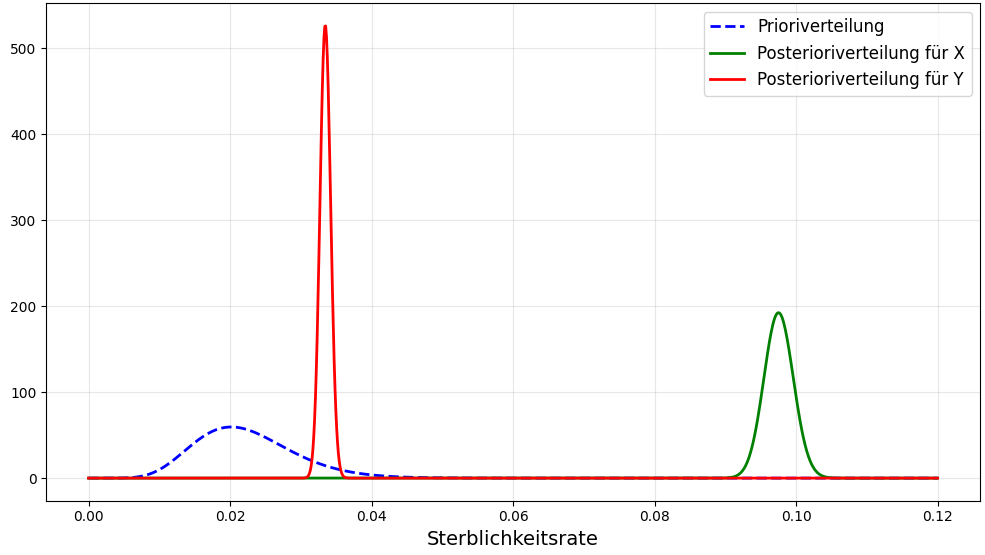
\includegraphics[width=0.85\textwidth]{../images/semmelweis.png}
\end{center}

Für $\alpha = 0.01$ beidseitige Konfidenzintervalle für $\Pi_X$ und $\Pi_Y$:
\begin{equation}
  I_X = [0.0927, 0.1034] \\
  I_Y = [0.0316, 0.0355]
\end{equation}

\subsubsection{Vergleich der Ergebnisse}
Der Vergleich der klassischen Statistik mit der bayesianischen Statistik liefert uns unterschiedliche Perspektiven:

\begin{itemize}
    \item Mit der klassischen Statistik haben wir die Sterblichkeitsraten für beide Perioden direkt berechnet und den Unterschied gemessen.
    \item Die bayesianische Statistik berücksichtigt zusätzlich Vorwissen und liefert eine schätzungsweise Wahrscheinlichkeitsverteilung 
    der Sterblichkeitsraten, was eine flexiblere Modellierung und Unsicherheitsabschätzung ermöglicht.
\end{itemize}
\newpage

\subsubsection{Vergleich der klassischen und bayesianischen Statistik}

\begin{table}[h!]
  \centering
  \begin{tabular}{|p{3cm}|p{5cm}|p{6cm}|}
    \hline
    \textbf{} & \textbf{Klassische Statistik} & \textbf{Bayesianische Statistik} \\ \hline
    \textbf{Bevorzugte Verwendung} & Human- und Sozialwissenschaften, Wirtschaftswissenschaften, Biologie & Technik und Künstliche Intelligenz \\ 
    \hline
    \textbf{Schätzen von Parametern, Testen von Hypothesen} & nur Stichprobe wird betrachtet & Stichprobe und Vorwissen wird betrachtet \\
    \hline
    \textbf{Ergebnis beim Schätzen} & Punkt- oder Intervallschätzer, z. B. Konfidenzintervall & Wahrscheinlichkeitsverteilung für den Parameter (Posterior) 
    \\ \hline
  \textbf{Ergebnis beim Testen} & \(p\)-Wert; Entscheidung basierend auf Signifikanzniveau, wird angenommen oder abgelehnt & Posterior-Wahrscheinlichkeit für Hypothesen; Bayes-Faktor \\ 
  \hline
  \end{tabular}
  \caption{Vergleich der klassischen und bayesianischen Statistik}
  \label{tab:vergleich_verwendung}
\end{table}

\begin{table}[h!]
  \centering
  \begin{tabular}{|p{4cm}|p{5cm}|p{5cm}|}
  \hline
  \textbf{Statistikmethode} & \textbf{Vorteile} & \textbf{Nachteile} \\ \hline
  \textbf{Klassische Statistik} & 
  \begin{itemize}
      \item Einfachheit und breite Akzeptanz in der Wissenschaft.
      \item Gut für große Datensätze und standardisierte Testverfahren.
      \item Benötigt keine subjektiven Annahmen über Wahrscheinlichkeiten.
  \end{itemize} & 
  \begin{itemize}
      \item Abhängig von großen Stichproben.
      \item Unflexibel gegenüber neuen Daten und Modellen.
      \item Ergebnisse oft schwer zu interpretieren bei komplexen Datenstrukturen.
  \end{itemize} \\ \hline
  \textbf{Bayesianische Statistik} & 
  \begin{itemize}
      \item Flexibel und anpassbar an komplexe Modelle.
      \item Ermöglicht die Einbeziehung von Vorwissen (Priors).
      \item Liefert direkte Wahrscheinlichkeiten für Parameter und Modelle.
  \end{itemize} & 
  \begin{itemize}
      \item Subjektivität bei der Wahl der Priors.
      \item Rechenintensiv, besonders bei großen Datensätzen.
      \item Oft weniger bekannt und akzeptiert in konservativen Disziplinen.
  \end{itemize} \\ \hline
  \end{tabular}
  \caption{Vergleich der Vor- und Nachteile der klassischen und bayesianischen Statistik.}
  \label{tab:vergleich_vor_nachteile}
\end{table}

\newpage

\section{Zusammenfassung und Ausblick}

\newpage

\section{Literaturverzeichnis} 

\printbibliography 
\newpage

\section{Selbstständigkeitserklärung}

\end{document}